\documentclass[10pt, a4paper, twoside]{amsart}

\usepackage[english]{babel}
\usepackage{amsthm,amssymb,amsmath,graphicx}
\usepackage{bbm}
\PassOptionsToPackage{hyphens}{url}\usepackage{hyperref}

\newcommand{\N}{\mathbb{N}}
\newcommand{\Z}{\mathbb{Z}}
\newcommand{\Q}{\mathbb{Q}}
\newcommand{\R}{\mathbb{R}}
\newcommand{\C}{\mathbb{C}}
\newcommand{\D}{\mathbb{D}}
\renewcommand{\a}{\alpha}
\renewcommand{\d}{\delta}
\newcommand{\p}{\partial}
\newcommand{\e}{\epsilon}
\newcommand{\w}{\omega}
\renewcommand{\l}{\lambda}
\newcommand{\vp}{\varphi}
\newcommand{\vn}{\emptyset}
\newcommand{\bs}{\backslash}
\newcommand{\A}{\mathcal{A}}
\newcommand{\F}{\mathcal{F}}
\renewcommand{\P}{\mathcal{P}}
\newcommand{\1}{\mathbbm{1}}
\newcommand{\im}{\textup{im}}
\renewcommand{\p}[2]{\frac{\partial #1}{\partial #2}}%partial
\renewcommand{\a}[1]{\left\lvert #1 \right\rvert}%abs
\renewcommand{\b}[1]{\left( #1 \right)}%brackets
\newcommand{\n}[1]{\left\lVert #1 \right\rVert}%norm

\newtheorem{definition}{Definition}
\newtheorem{lemma}{Lemma}
\newtheorem{theorem}{Theorem}

\newcommand\textbox[1]{
  \parbox{.333\textwidth}{#1}}

\newcommand{\homeworkset}{}
\newcommand{\courseName} {A3.6 Maze Generation}
\newcommand{\firstName}  {Wouter}
\newcommand{\lastName}   {Slegers}
\newcommand{\studId}     {19950825-1957}
\renewcommand{\email}    {wjslegers@gmail.com}

\pagestyle{plain}
\begin{document}
\noindent{\huge\bf \courseName}\\
\noindent\textbox{\sc \firstName~ \lastName \hfill}\textbox{\hfil Uppsala University \hfil}\textbox{\hfill \studId}
\noindent\textbox{\large\sc Report \hfill}\textbox{\hfil \today \hfil}\textbox{\hfill \email}
\bigskip


\section*{Introduction}
I have elected to do project A3.6 and make a maze generation algorithm. I came up with three different algorithms. The first a search algorithm, the second is inspired by random walks and the last one is inspired by evolutional teaching of AI to play games. The latter is not very suitable for the purpose nor recursive but fun to work with!

\subsection*{Practical information}
I use the word maze for any set of fields arranged in a square, with walls around the edges and each field is connected to its horizontal or vertical neighbours either by a 'wall' or an 'opening'. We may speak of fields being connected or not depending on a wall being there. Also I use the words node and field interchangeably.
I set the goal of a 'correct maze' as a maze that has a path of connections from the top left to the bottom right. In the code that is from field \verb+(0, 0)+ to field \verb+(maze.fields - 1, maze.fields - 1)+, where \verb+maze.fields+ is the number of fields of maze. The goal is to create an algorithm that makes such a 'correct maze', preferably with as many walls still standing, one could after all just remove all walls and be done with it, but be left with a rather boring maze.\\

To make writing code as easy as possible I chose Python, as I find it quick and easy to set things up. 
You can find all the Python files in the zip-folder.
I made a 'Maze' class and print it using the 'print()' function of Python to simplify the creating of the graphical part of the program.


\section{Path Through Maze Algorithm}
The idea of the algorithm is to first generate a relatively dense random maze. For example, for each wall there is a $70\%$ chance it becomes a wall and $30\%$ it is left open. Then we use a search algorithm that saves all the nodes it can reach from the starting node in a list called \verb+searched+. Every node that is a dead end it also saves in a list called \verb+dead_ends+, a dead end we define as a node with three or more walls around it. We go through the dead ends until we find one that has a wall that leads to a previously unexplored node i.e. the neighbouring node is not in \verb+searched+. We make a connection and the algorithm repeats the search from the new node. We keep the \verb+searched+ and \verb+dead_ends+ lists, the latter minus the newly opened up dead end. This way we 'search' each node only once and the time the algorithm takes stays limited. We end when all nodes are searched.

\subsection{Why it works}
The idea is that the algorithm will not stop searching the maze and opening up connections until there is a path that reaches the end ensuring that it gives a correct maze. However, it is possible that there are no suitable dead ends during one of the steps in the algorithm. See the figure below with such an example. On the right is the same maze but with the fields marked 's' for searched or 'd' for searched and a dead end. When this situation arises we take a randomly selected previously searched node, that is not necessarily a dead end, but has an unsearched neighbour.

\begin{figure}
\centering
        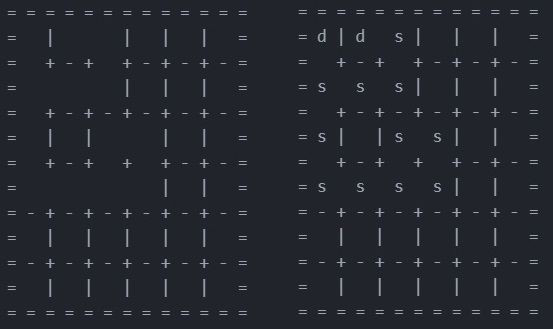
\includegraphics[totalheight=8cm]{nodeadends}
    \caption{Example of a maze without suitable dead ends}
\end{figure}

\subsection{Tweaks to the algorithm}
There are some choices we can make.
We have a choice of which dead end we open up in each step (or alternatively which searched node we open up) and a choice of which neighbour we open it up to.
I chose to favour opening up dead ends further away from the diagonal line between the beginning and end, to encourage creating longer paths, with the following line of code.\\
\verb+dead_ends.sort(reverse=True, key=lambda node: abs(node[0] - node[1]))+\\
After this we take the first suitable dead end we find in the list. For the choice of neighbour we go with a random one. Also if we need to open a searched node instead of searched dead end, it is picked randomly.
Another important choice is the begin density of the maze. Make it too open and there'll already be some paths to the end, and a sparse maze isn't the most interesting. Choosing density $1$, i.e. all walls are up, this algorithm becomes more or less a random walk algorithm due to the choices above. However each step is a recursive call so the size of the maze would have to stay under $31$ by $31$ to steer clear of Python's default recursive call limit of $997$. Having the begin density parameter gives some customisability to the algorithm.

\subsection{Notes on the algorithm}
To run the generation just execute \verb+PathThroughMaze.py+. The variables \verb+SIZE_MAZE+ and \verb+BEGINNING_DENSITY+ can be played around with. Whether we print the steps in between can be changed with the boolean \verb+PRINTING_STEPS+. When printing the maze you can use \verb+maze.print(False)+. False indicates that you want to leave the fields empty. With True it also prints the fields, which during the execution of the algorithm get marked with 's' if they've been searched, which in turn can get overridden by 'd' for dead ends or 'O' if it is a node that has been opened.\\


\section{Self-avoiding random walk}
When I worked on this algorithm I must have forgotten that a very similar method 'hunt and kill' was already discussed in the slideshow linked in the project description together with the improved version 'recursive backtracker'. I'd still like to include my version here!
The idea of this algorithm is to start a self-avoiding random walk from the beginning of the maze, leaving a path of connections through an initially fully walled in maze. Whenever it can make no further steps we repeat, we start from a previously visited node that has an unvisited neighbour. We don't stop until  every node has been visited. This results in a fully connected maze. In the figure below we give an example of the first two steps in the algorithm. When the boolean \verb+PRINTING_STEPS+ is True we mark newly visited nodes with 'n', the node where the latest path ends is marked with 'e' and nodes visited in previous steps are replaced by 'v'.

\begin{figure}
\centering
        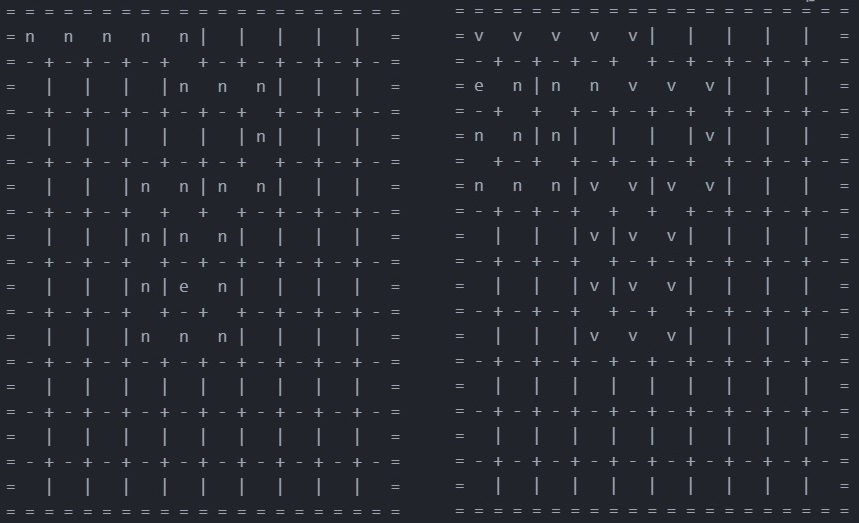
\includegraphics[totalheight=8cm]{beginwalker}
    \caption{Two steps of the walker maze generation algorithm creating a $10$ by $10$ maze}
\end{figure}


\subsection*{Notes on the algorithm}
To run the generation just execute \verb+Walker.py+.

The algorithm is the quickest of the three, since nodes get visited once, and not many other calculations happen. It always gives a fully connected maze and the paths are, as you might suspect, rather random.

Each path created is another recursive call, so creating very large mazes may have you reach the maximum recursion depth, but it is still faster and capable of much larger mazes than the path-through-maze algorithm with begin density $1$.


\section{Evolutional learning}
I considered suggesting a project on evolutional learning of neural networks, but instead ended up doing the maze generation project. However, borrowing from that I had an idea for another maze generation algorithm.\\
We create a certain amount of random mazes. We give each a score and take the best mazes from this generation to go to the next generation. Each of those mazes creates a few mutations of itself to also be tested in that next generation. Like in natural evolution, if the random mutations turn out to be beneficial they 'survive' to the next generation.\\
This requires a lot of tuning of parameters, such as how the mutations happen and most importantly how the mazes get scored.

\subsection{Performance of the algorithm}
This is a very memory and computationally expensive way of creating mazes, so not the most practical. To create good mazes it seems to help to have some sort of search algorithm integrated in the scoring function. But since the scoring function gets called so very often, that makes this method quite computationally expensive.
Furthermore there is no guarantee that the algorithm finishes with a maze that has a path from beginning to finish. However by strongly increasing scores for mazes that have a path from start to finish and running enough generations we can make it extremely likely that it does deliver a correct maze.

\subsection{Notes on the algorithm}
I made two versions, \verb+Evolutionary.py+ and\\ \verb+EvolutionaryLongPath.py+.
The first uses a scoring function that creates a list of nodes that can be reached from the beginning node, using the \verb+distance_to_end+ function. If none of the reachable nodes are close to the end the score will be low. Also a high number of nodes that can not be reached decreases the score. To prevent making the maze too sparse the score is increased slightly for each wall it has. The downside of this method is that the maze it produces often has a rather short path to the end.
The other version, \verb+EvolutionaryLongPath.py+, is meant to prevent that. Here, in the scoring function, we use a search function \verb+shortest_path+ that keeps track of shortest distance from the start node to each node in the maze. This way we can also punish for nodes that can not be reached and reward for reaching the last node. But now we can also give higher scores to mazes that have a long path to the end instead of a short one! This creates, what I consider to be, more interesting mazes. Again we give a slightly higher score for mazes with more walls.\\
Once a maze is found that reaches the end, the large majority of the mutated children are worse mazes, and the progress becomes very slow. So to fully utilise this and give it more time to create a longer path we can use more generations.

The second version uses a recursive search algorithm that could potentially go through every node and even the same node multiple times if it finds a shorter path there. So for mazes larger than $30$ by $30$ there is potential for recursive call depth errors, however this type of algorithm is unsuitable for large mazes anyway since it would take a lot of generations to find a good maze. The latter algorithm in particular is unsuitable for large mazes since the score does not account for being closer to making a path to the end like the first version does.
In testing both versions tend to create decent mazes of size $12$ by $12$ in as few as $30$ generations, with $80$ mazes in each generation. 


\end{document}